\section{Air Quality}
\subsection{Air pollution and its health effects}
Air pollution can be defined as a group of chemicals present in the atmosphere that are harmful to humans, animals or vegetation. It is mainly caused by human activities, such as transport, industry, or agriculture. But it can also be influenced by other natural sources. Understanding air pollution is important because many health consequences result from high pollution levels. 
\begin{figure}[h]
  \centering
  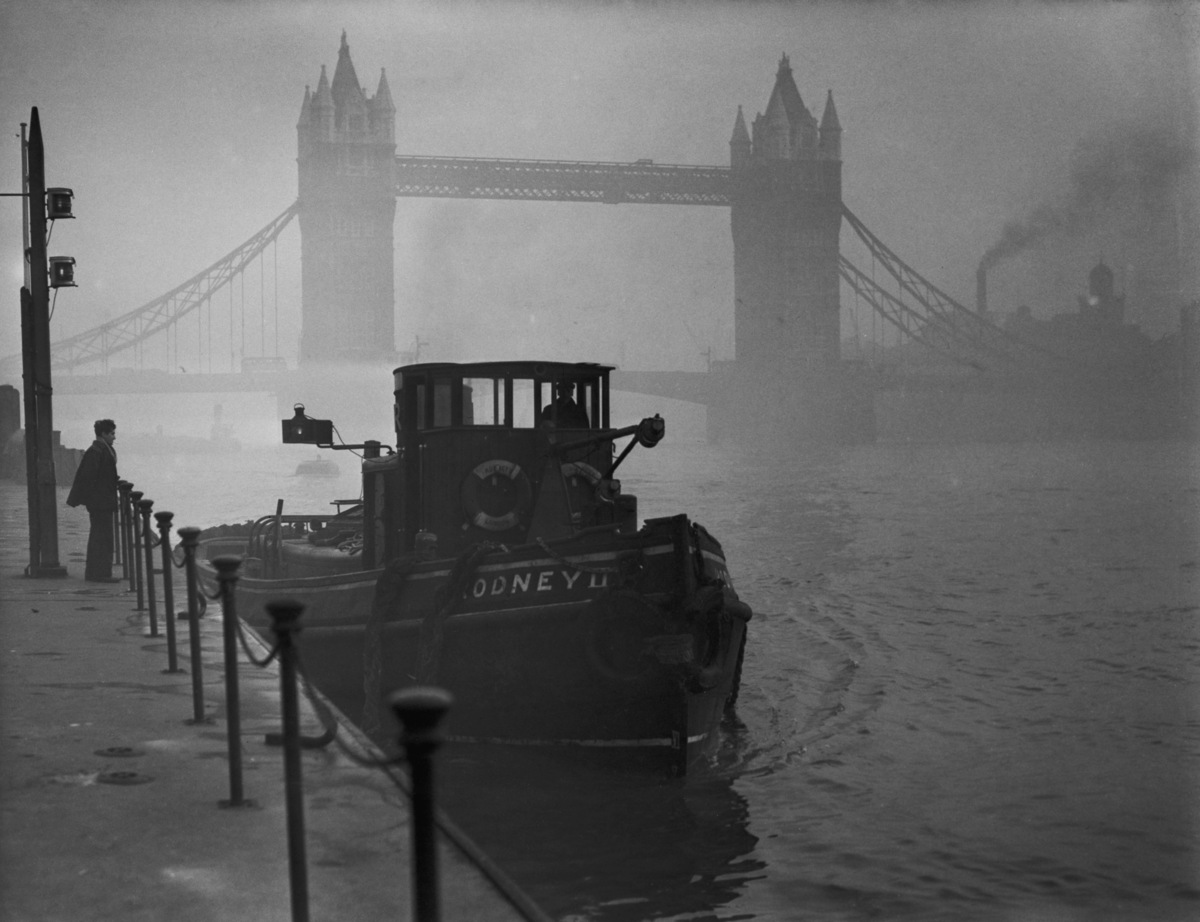
\includegraphics[scale=.8]{images/great_smog.jpg}
  \caption[Great smog of 1952]{Great smog of 1952 \cite{ElliotWagland2013}}
  \label{fig:interaction_design}
\end{figure}

One historic event which caused huge consequences is known as the great smog of 1952. Thousands of people died in Greater London due to exposure over several days to a highly contaminated atmosphere, and many others became ill or experienced retarded symptoms \cite{Bell2008}. The fog originated from coal burning, vehicle exhaust and other atmospheric factors. Although many human activities introducing pollution have changed since then, it became evident the immediate and retarded health impact of pollution. 

Pollution particles can be categorised into gaseous pollutants, persistent organic pollutants, heavy metals and particulate matter. They vary in their chemical composition, emission sources and impact on health. 

Gaseous pollutants are sulphur dioxide (\SOTWO), nitrogen oxides (\NOX), carbon monoxide (CO), ozone (\OTHREE) and volatile organic compounds (VOCs). The principal source of gaseous pollutants is combustion of fossil fuels and diesel emission from vehicles. Nitrogen oxides (\NOX) is a general term that includes nitric oxide (NO) and nitrogen oxide \NOTWO. Gaseous pollutants can affect our health by inflaming the airways and lungs, and in the long term, affect the function of the lungs \cite{AirQualityExpertGroup2004} \cite{WHO2003}.

Particulate matter (PM) is a mixture of solid and liquid particles (such as sulphate, nitrates, ammonia, sodium chloride, black carbon, mineral dust and water). PM are categorised according to their diameter size measured in microns (\SI{}{\micro\metre}, one millionth of a metre). Particles smaller than 10 microns (\PMTEN) are known as coarse particles, smaller particles with a size of up to 2.5 and 1 microns (\PMTWO and \PMONE) are known as fine and ultra-fine particles respectively. They are differentiated in sizes because it dictates their aerodynamic properties, that is, how they are transported into the air, as well as how far they can get into the respiratory system. According to the World Health Organization, PM is the most harmful pollutant because it can pass through the nose and throat and enter the lungs, there is also evidence that it is associated with risk of cardiovascular disease \cite{Polichetti2009}. 

Air quality is also affected by pollution mixture in further complex chemical structures and by temperature and humidity conditions. \NOTWO, PM and O\textsubscript{3}  pollutants get transformed by atmospheric processes making it hard to evaluate their individual impact. As an example, ground level ozone is produced when sunlight interacts with \NOTWO and volatile organic compounds. Furthermore, \NOTWO and other nitrogen oxides also contribute to PM generation, making \NOX a particularly concerning pollutant.

\subsection{Air quality data dissemination}
Openly published air quality data aimed to have informed and aware citizens that could take part into more sustainable and environmental choices. \quotes{Yet, what was lacking (and it still is), is a model for effective communicating of environmental information to the public} \cite{Thinh2007}. Terms like assessment, limit values, target values and concentration, among others, are commonly used by air quality data publishers to describe the current or forecasted quality status; however, there is not general agreement on how air quality information should be disseminated to the general public in a way it is understood immediately and intuitively. 

In general it is complex to categorise and establish measures for the different components of air pollution due their heterogeneous nature and the chemical reactions that occur between them. Measurement methods and units vary from institution to institution and regulation standards can be specific for each country, which may give rise to ambiguity. Furthermore, much of the available data is represented in a tabular format, including various information for individual pollutants, as exemplified in table \ref{tab:pollution_tabular_data}. This table was extracted from the  Department for Environment Food and Rural Affairs (DEFRA) website \cite{DepartmentforEnvironmenta}, and shows measures related to the air quality from a sensing station located in Deaconess Garden in the south of Edinburgh. At first sight it table arises some questions for the novice on air-quality trying to crack the data. Firstly, the pollution codes such as PM2.5, PM10, NO2, NOX as NO2 and their subtle differences should be understood. Secondly, some measurement units are tagged with the monitoring method used to extract the information, like the TEOM FDMS \footnote{Which indicates that the sensing methods were Tapered Element Oscillating Microbalance and Filter Dynamics Measurement System \cite{Quality2005}} tag. And lastly, it is hard to know which measurements are of more interest given a person's particular circumstances. As stated by Brimblecombe and Schuepbach \cite{P.Brimblecombe2008}, \quotes{many people complain that the information is unintelligible, while some have even seen it as an attempt of government to blind the public with science}.  It is clearly difficult to understand the meaning of the terms and values that are used to represent air quality data to the general public. 

\begin{table}[ht]
\centering
\begin{adjustbox}{width=1.2\textwidth,center=\textwidth}
\begin{tabular}{rlrrrrrrr}
  \hline
 Pollutant & Date & Time & Measurement & Unit & Period & Comment  \\ \hline
    Ozone (O3) & 20/07/2016 & 07:00 & 63.06412 & µg/m3 & Hourly & - \\
    Nitric oxide (NO) & 20/07/2016 & 07:00 & 2.61933 & µg/m3 & Hourly & - \\
    Nitrogen dioxide (NO2) & 20/07/2016 & 07:00 & 27.34875 & µg/m3 & Hourly & - \\
    Nitrogen oxides as nitrogen dioxide (NOXasNO2) & 20/07/2016 & 07:00 & 31.36500 & µg/m3 & Hourly & - \\
	Sulphur dioxide (SO2) & 20/07/2016 & 07:00 & 14.63495 & µg/m3 & Hourly & - \\
	Carbon monoxide (CO) & 20/07/2016 & 07:00 & 0.081494 & mg/m3 & Hourly & - \\
	PM10 particulate matter (Hourly measured) (PM10) & 18/07/2016 & 15:00 & 10.900 & µg/m3 (TEOM FDMS) & Hourly & - No current data. \\
	Non-volatile PM10 (Hourly measured) (Non-volatile PM10) & 19/07/2016 & 07:00 & 26.700 & µg/m3 (TEOM FDMS) & Hourly & - No current data. \\
	Volatile PM10 (Hourly measured) (Volatile PM10) & 19/07/2016 & 07:00 & 5.500 & µg/m3 (TEOM FDMS) & Hourly & - No current data. \\
	PM2.5 particulate matter (Hourly measured) (PM2.5) & 18/07/2016 & 15:00 & 4.300 & µg/m3 (TEOM FDMS) & Hourly & - No current data. \\
	Non-volatile PM2.5 (Hourly measured) (Non-volatile PM2.5) & 19/07/2016 & 07:00 & 16.300 & µg/m3 (TEOM FDMS) & Hourly & - No current data. \\
	Volatile PM2.5 (Hourly measured) (Volatile PM2.5) & 19/07/2016 & 07:00 & 5.000 & µg/m3 (TEOM FDMS) & Hourly & - No current data. \\
	Modelled Wind Direction (Dir) & 19/07/2016 & 24:00 & 50.6 & \degree & Hourly & - No current data. \\
	Modelled Wind Speed (Speed) & 19/07/2016 & 24:00 & 6.2 & m/s & Hourly & - No current data. \\
	Modelled Temperature (Temp) & 19/07/2016 & 24:00 & 14.6 & °C & Hourly & - No current data. \\
	PM10 Ambient Temperature (AT10) & 19/07/2016 & 07:00 & 19.4 & °C & Hourly & - No current data. \\
	PM10 Ambient pressure measured (AP10) & 19/07/2016 & 07:00 & 989.0 & mb & Hourly & - No current data. \\
	PM2.5 Ambient Temperature (AT25 ) & 19/07/2016 & 07:00 & 17.5 & °C & Hourly & - No current data. \\
	PM2.5 Ambient Preasure (AP25) & 19/07/2016 & 07:00 & 988.0 & mb & Hourly & - No current data. \\
   \hline
\end{tabular}
\end{adjustbox}
\caption{Air quality tabular data representation. \cite{DepartmentforEnvironment}}
\label{tab:pollution_tabular_data}
\end{table} 

\subsection{The COMEAP air quality index and health advice}
In order to understand the correlation between air quality data and its effects on human health, the Committee on the Medical Effects of Air Pollutants (COMEAP) developed the air quality index based on health evidence. It is used to communicate real-time air quality levels and their short-term health effects for five selected harmful pollutants: particulate matter (\PMTEN and \PMTWO), ozone (\OTHREE), sulphur dioxide (\SOTWO), and nitrogen dioxide (\NOTWO) as shown in Figure \ref{fig:air_quality_index}. The index employs a colour scale and a number index to inform about how high are the concentrations of each specific pollutant. Four bands are employed: Low, Moderate, High and Very High. 

\begin{figure}[H]
\begin{adjustbox}{width=1\textwidth,center=\textwidth}
  \centering
  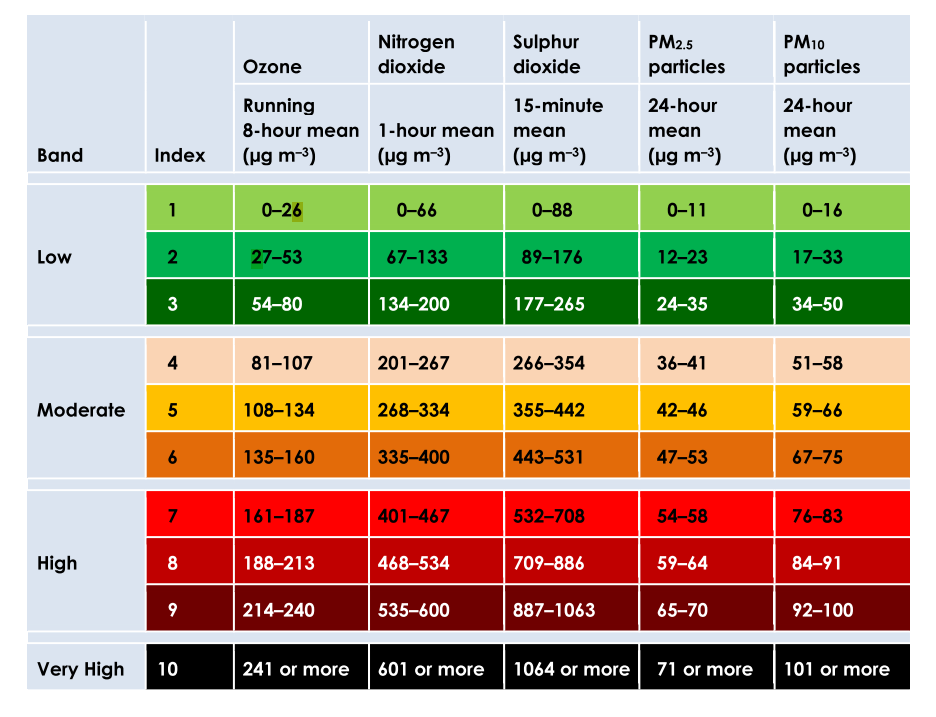
\includegraphics[scale=.8]{images/air_quality_index.png}
\end{adjustbox}
  \caption[The COMEAP air quality index]{The COMEAP air quality index \cite{HealthProtectionAgencyfortheCommitteeontheMedicalEffectsofAirPollutants2011}}
  \label{fig:air_quality_index}
\end{figure}

There is substantial evidence that the elderly, children, and persons that suffer from chronic diseases such as asthma are in greater danger of suffering symptoms and health consequences from lower pollution concentrations than the general public \cite{Koenig1999} \cite{Kampa2008} \cite{Zones2010} . The COMEAP includes such population in their Air Quality Index to give them the opportunity to modify their behaviour and reduce the severity of their symptoms. Furthermore, the air quality index is accompanied by a health advice (Figure \ref{fig:air_quality_health_advice}) which provides specific health messages targeting both population groups, sensitive and non-sensitive providing information about the actions that should be taken to avoid symptoms and health effects.

\begin{figure}[H]
\begin{adjustbox}{width=1\textwidth,center=\textwidth}
  \centering
  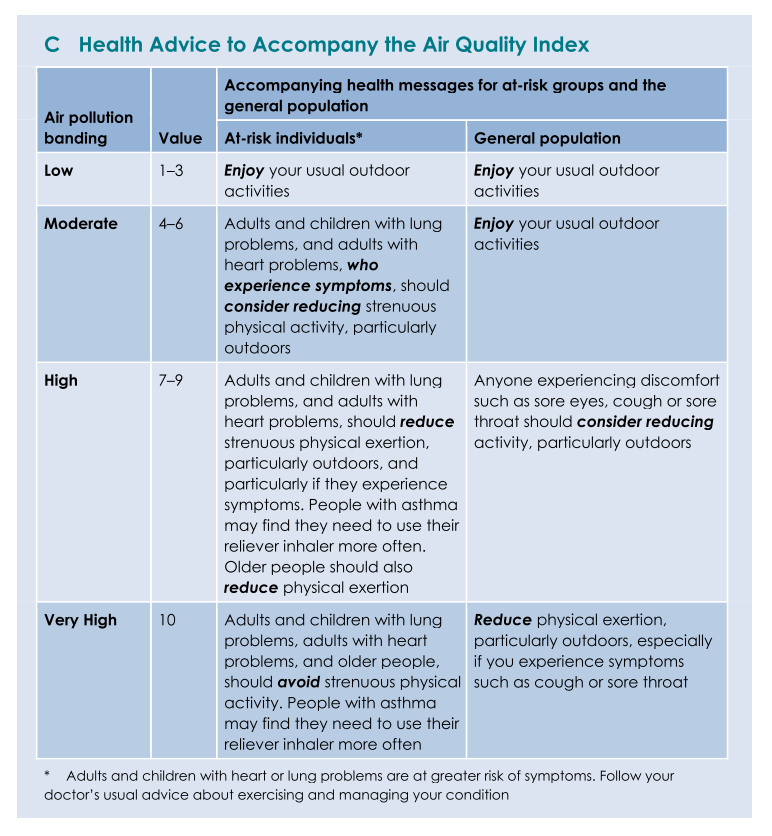
\includegraphics[scale=.8]{images/air_quality_health_advice.png}
\end{adjustbox}
  \caption[Air quality health advice]{Air quality health advice \cite{HealthProtectionAgencyfortheCommitteeontheMedicalEffectsofAirPollutants2011}}
  \label{fig:air_quality_health_advice}
\end{figure}


\subsection{Air quality sensors}

\begin{itemize}

\item Fixed sensors: 

Fixed sensors are installed and maintained by the UK government and local authorities in Scotland. There are of two kinds, automatic sensors from the Automatic Urban and Rural Network (AURN)\footnote{\url{https://uk-air.defra.gov.uk/networks/network-info?view=aurn}}, and non automatic sensors maintained by local Scottish councils. 

	\begin{itemize}
    
    \item Automatic sensors: They produce hourly concentrations and data is sent automatically over the network. They purpose is to check that EU and other regulatory standards are being met as well as informing the public about air quality. These sensors monitor a wide range of pollutants (\NOX, \SOTWO, CO\textsubscript{2}, O\textsubscript{3}, \PMTWO and \PMTEN) which are later collected and processed by Ricardo Energy and Environment \footnote{\url{http://ee.ricardo.com}} and exposed through HTML webpages at the Scottish Air Quality website\footnote{\url{http://www.scottishairquality.co.uk/}} or CSV files provided on demand. 
	\item Non automatic sensors: 
    
    \end{itemize}

\item Portable sensors:

\item Participatory sensors:

Some projects such as CitiSense \cite{Nikzad2012} include users as 'human sensors' by reading their perceptions towards air quality in certain locations. This method aims to get more fine-grained information about air quality and engage the citizens in the pollution problem and its solution. 

\end{itemize}



